\section{M3 results and interpretation}
\subsection{Prediction: several approaches under common splits}
\begin{table}[!htbp]\centering\small
\begin{tabular}{@{}lrrr@{}}\toprule
Method & RMSE & MAE & NLL\\\midrule
Global & 1.1164 $\pm$ 0.0021 & 0.9334 $\pm$ 0.0018 & 1.4552 $\pm$ 0.0015\\
User mean & 1.0342 $\pm$ 0.0021 & 0.8303 $\pm$ 0.0020 & 1.3461 $\pm$ 0.0016\\
Item mean & 0.9786 $\pm$ 0.0026 & 0.7826 $\pm$ 0.0021 & 1.3209 $\pm$ 0.0028\\
MF-SGD & 0.8683 $\pm$ 0.0024 & 0.6906 $\pm$ 0.0023 & 1.2214 $\pm$ 0.0025\\
ADF / EP1 & 0.8977 $\pm$ 0.0035 & 0.7098 $\pm$ 0.0030 & 1.2519 $\pm$ 0.0033\\
EP3 & 0.8740 $\pm$ 0.0036 & 0.6894 $\pm$ 0.0026 & 1.2283 $\pm$ 0.0033\\
EP5 & 0.8643 $\pm$ 0.0037 & 0.6808 $\pm$ 0.0025 & 1.2189 $\pm$ 0.0035\\
EP10 & 0.8548 $\pm$ 0.0029 & 0.6721 $\pm$ 0.0018 & 1.2098 $\pm$ 0.0024\\
MF-MAP (no graph) & 0.8506 $\pm$ 0.0021 & 0.6753 $\pm$ 0.0017 & 1.2012 $\pm$ 0.0021\\
GMRF-MAP & 0.8499 $\pm$ 0.0023 & 0.6752 $\pm$ 0.0019 & 1.2007 $\pm$ 0.0024\\
\bottomrule\end{tabular}

\caption{Fresh full MovieLens 1M results, mean $\pm$ sample SD over seeds 42--46.
Every row uses the expected star rating. Lower is better.}
\label{tab:m3main}
\end{table}
The fresh ADF/EP5 scores for seeds 42--44 reproduce the M2 values; differences
in the new aggregate arise from adding seeds 45 and 46, not from replacing
the old dataset with the synthetic demo. ADF/EP1 have identical natural
parameters. Repeated inference improves mean RMSE from 0.8977 to 0.8643 at EP5
and 0.8548 at EP10. This supports revisiting evidence with cavity removal,
at increased computational cost. Ten passes remain a finite budget, not a
proof of convergence.

GMRF-MAP reaches 0.8499, compared with 0.8643 for EP5 and 0.8548 for EP10.
The corresponding reductions are about 1.67\% and 0.57\%.
These are \emph{whole-system} comparisons: Gaussian numeric-rating training,
MAP fitting and regularization differ from ordinal EP. The stronger graph-free
MF-MAP baseline already reaches 0.8506. Therefore most of the gain over EP5
cannot be attributed solely to adding a network.

Conventional MF-SGD remains a useful inexpensive baseline. Its expected-rating
RMSE is 0.8683, while its separately decoded clipped score gives 0.8650.
For MF-MAP and GMRF-MAP, clipped-score RMSE is 0.8478 and 0.8465, respectively.
Those numbers are supplied as secondary decoding results; the main table uses
one common expected-rating definition. Mean-only models have larger error,
supporting the value of personalization on this random-interaction benchmark.

\begin{figure}[!htbp]\centering
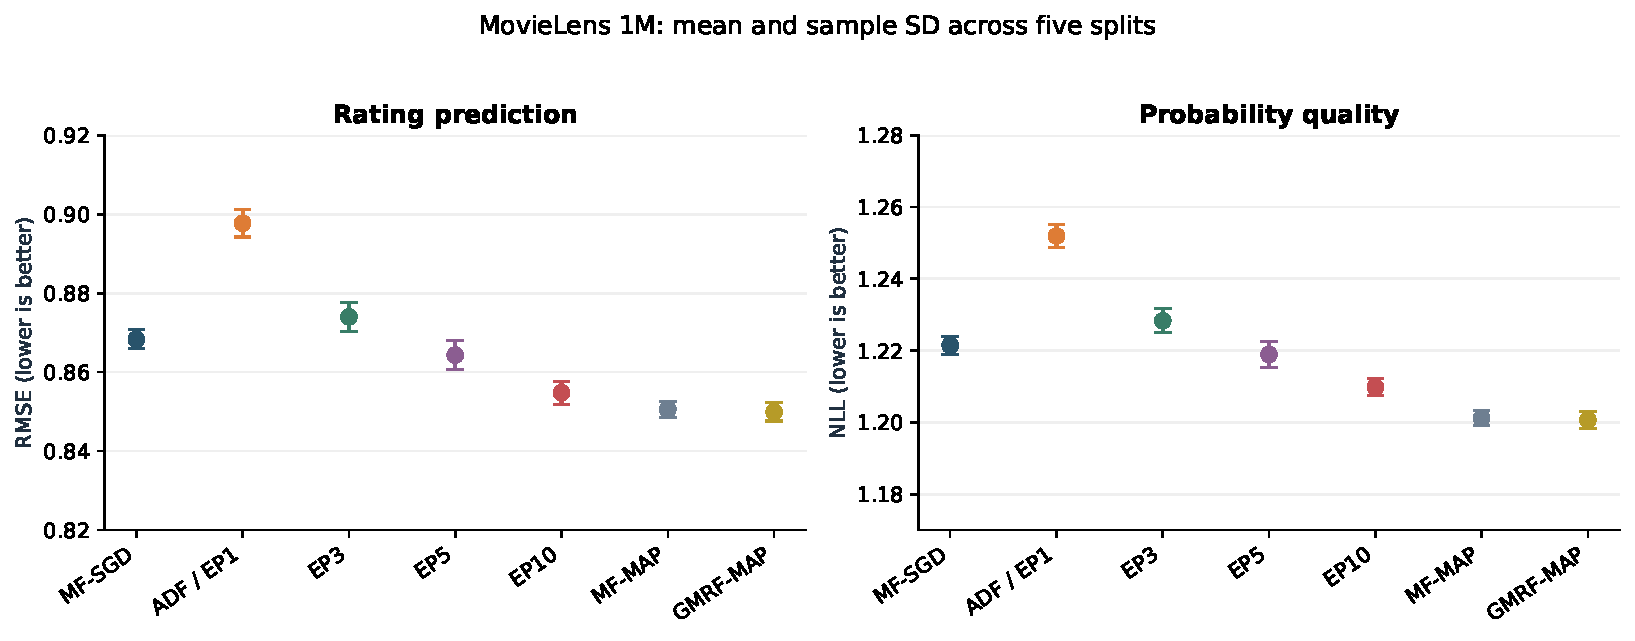
\includegraphics[width=\linewidth]{../../Results/analysis/plots/main_comparison.pdf}
\caption{Accuracy and probability quality. Error bars are sample SD over five
splits, not confidence intervals. The vertical scales are restricted for readability.}
\end{figure}

\subsection{What improvement is actually due to the Markov prior?}
All five clean-validation searches select $\gamma=10$ over 0, 1 and 100.
Against the matching $\gamma=0$ model, the graph reduces mean expected-rating
RMSE by 0.000644 (approximately 0.076\%). The point estimate improves in every
split, but the effect is small in practical star units.

\begin{table}[!htbp]\centering\small
\begin{tabular}{@{}lrr@{}}\toprule
Seed & RMSE reduction & 95\% user-bootstrap interval\\\midrule
42 & +0.000941 & [+0.000562, +0.001330]\\
43 & +0.000380 & [-0.000044, +0.000833]\\
44 & +0.000492 & [+0.000061, +0.000890]\\
45 & +0.000503 & [+0.000070, +0.000937]\\
46 & +0.000906 & [+0.000148, +0.001726]\\
\bottomrule\end{tabular}

\caption{MF-MAP minus GMRF-MAP expected-rating RMSE. Positive means the graph
helps. Intervals use paired user resampling within each fitted split.}
\label{tab:graphci}
\end{table}
Four split-specific intervals lie above zero; seed 43 includes zero. The
conditional bootstrap therefore provides support in several splits without
establishing a universal or independent-replication significance claim.
The NLL difference is also small, and its interval includes zero for several
splits (full table in the results files). We do not claim improved calibration
from the graph: mean ECE changes from 0.03835 to 0.03868, slightly worse.

\begin{figure}[!htbp]\centering
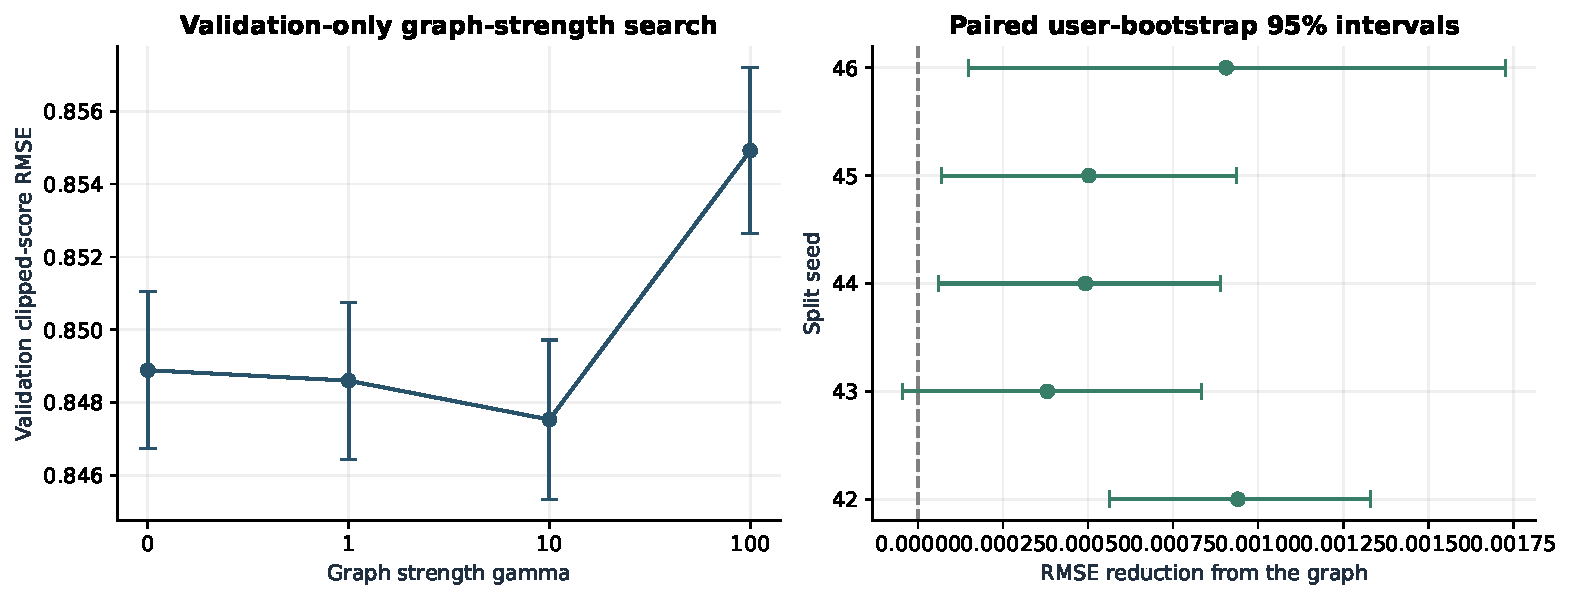
\includegraphics[width=\linewidth]{../../Results/analysis/plots/graph_evidence.pdf}
\caption{Graph-strength validation and the paired graph-only test effect.
Strength 100 worsens validation error; stronger smoothing is not always better.}
\end{figure}

The mechanism is consistent with modest regularization: neighbouring movie
vectors share evidence while the data term retains personalization. The
ablation establishes the effect of this prior \emph{within this solver and
selection protocol}; it does not prove that the selected neighbours are true
dependencies or explain each gain causally. The stress tests below examine
where this explanation remains useful and where it fails.

\subsection{Probability quality and the two noise questions}
\begin{table}[!htbp]\centering\small
\begin{tabular}{@{}lrrr@{}}\toprule
Method & Brier & ECE & Star accuracy\\\midrule
MF-SGD & 0.6554 $\pm$ 0.0011 & 0.0397 $\pm$ 0.0010 & 46.04 $\pm$ 0.16\%\\
ADF / EP1 & 0.6681 $\pm$ 0.0012 & 0.0451 $\pm$ 0.0010 & 44.13 $\pm$ 0.13\%\\
EP3 & 0.6590 $\pm$ 0.0012 & 0.0537 $\pm$ 0.0017 & 45.20 $\pm$ 0.18\%\\
EP5 & 0.6552 $\pm$ 0.0012 & 0.0566 $\pm$ 0.0009 & 45.59 $\pm$ 0.16\%\\
EP10 & 0.6516 $\pm$ 0.0007 & 0.0608 $\pm$ 0.0012 & 46.04 $\pm$ 0.21\%\\
MF-MAP (no graph) & 0.6467 $\pm$ 0.0007 & 0.0383 $\pm$ 0.0018 & 46.98 $\pm$ 0.15\%\\
GMRF-MAP & 0.6468 $\pm$ 0.0009 & 0.0387 $\pm$ 0.0022 & 46.96 $\pm$ 0.19\%\\
\bottomrule\end{tabular}

\caption{Probability quality and exact-star accuracy (percent), five-seed
mean $\pm$ SD. Accuracy uses the most probable star, not rounded expected stars.}
\end{table}
More EP passes improve RMSE, NLL and Brier, but worsen ECE: 0.0451 for ADF,
0.0566 for EP5 and 0.0608 for EP10. Thus lower rating error does not mean more
calibrated confidence. A global empirical distribution has low ECE but poor
personalized error, illustrating that calibration alone is insufficient.
GMRF-MAP has better NLL than EP5/EP10 here, while its probability model still
omits posterior parameter uncertainty. Nominal 90\% equal-tail intervals
cover 98.22\% of ratings for EP5 and 97.41\% for GMRF-MAP, with mean
widths 3.82 and 3.60 star categories. Such broad, discrete intervals should not
be advertised as well calibrated merely because their coverage is high.

\begin{figure}[!htbp]\centering
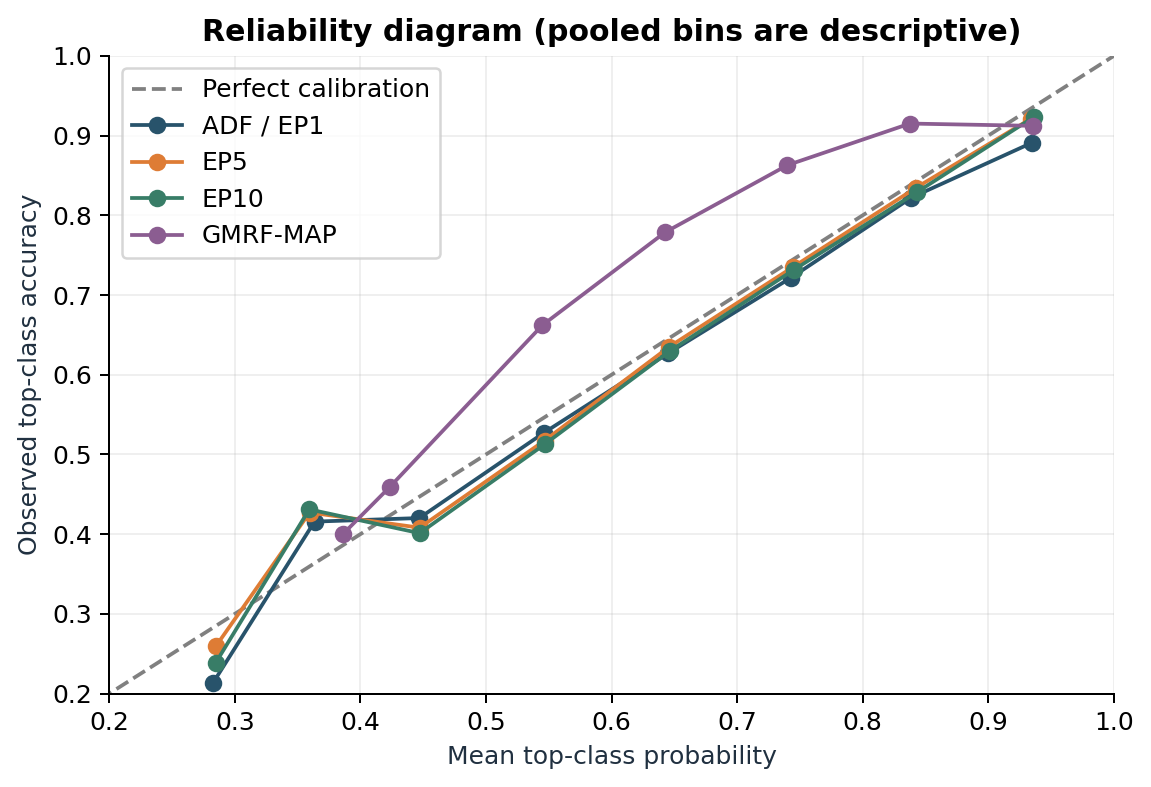
\includegraphics[width=.84\linewidth]{../../Results/analysis/plots/reliability.png}
\caption{Top-class reliability. Pooling overlapping split bins is descriptive;
the curve is not an independent-data significance analysis.}
\end{figure}

\begin{table}[!htbp]\centering\small
\begin{tabular}{@{}lrrr@{}}\toprule
Noise variance & RMSE & NLL & ECE\\\midrule
0.5 & 0.8691 $\pm$ 0.0036 & 1.2404 $\pm$ 0.0054 & 0.0339 $\pm$ 0.0012\\
1.0 & 0.8643 $\pm$ 0.0037 & 1.2189 $\pm$ 0.0035 & 0.0566 $\pm$ 0.0009\\
2.0 & 0.8743 $\pm$ 0.0030 & 1.3154 $\pm$ 0.0020 & 0.0856 $\pm$ 0.0012\\
\bottomrule\end{tabular}

\caption{EP5 observation-noise variance sensitivity. This changes the assumed
likelihood variance, not the dataset's labels.}
\end{table}
Validation NLL chooses $\beta^2=1$ in every seed. Halving it improves ECE to
0.0339 but worsens NLL to 1.2404 and RMSE to 0.8691. Doubling it worsens all
three displayed measures. A smaller assumed variance sharpens probabilities;
the data do not support a blanket claim that reducing noise always improves
inference. The separate label-corruption experiment measures resistance to
wrong training observations while keeping evaluation labels unchanged.

\subsection{Computational cost, convergence and exact-reference checks}
\begin{table}[!htbp]\centering\small
\begin{tabular}{@{}lrrr@{}}\toprule
Method & Fit (s) & Predict ($\mu$s/rating) & Site MiB\\\midrule
MF-SGD & 1.38 $\pm$ 0.04 & 0.413 & 0\\
ADF / EP1 & 3.33 $\pm$ 0.19 & 0.810 & 0\\
EP3 & 10.99 $\pm$ 0.57 & 0.749 & 219.77\\
EP5 & 18.29 $\pm$ 2.02 & 0.679 & 219.77\\
EP10 & 35.99 $\pm$ 6.61 & 0.779 & 219.77\\
MF-MAP (no graph) & 16.74 $\pm$ 2.74 & 0.449 & 0\\
GMRF-MAP & 14.48 $\pm$ 1.82 & 0.487 & 0\\
\bottomrule\end{tabular}

\caption{Selected-candidate fitting and batch prediction cost; mean $\pm$ SD
where shown. EP site memory is an array-size calculation, not process RSS.}
\end{table}
EP5 takes about 5.49 times ADF's mean fit time; EP10 about 10.81 times.
Both repeated-EP budgets use the same 219.77 MiB cache at $K=8$; more passes
increase time rather than site count. MF-SGD fits in about 1.38 seconds under
this implementation. Mean graph construction takes 4.31 seconds and the full
four-candidate MAP search takes 66.37 seconds, beyond the selected GMRF
candidate's 14.48 seconds. A claim that GMRF is simply ``faster than EP'' would
ignore this search/setup cost. Selected MAP wall times vary despite equal epoch
budgets; they do not establish an intrinsic speed advantage from graph edges.

\begin{figure}[!htbp]\centering
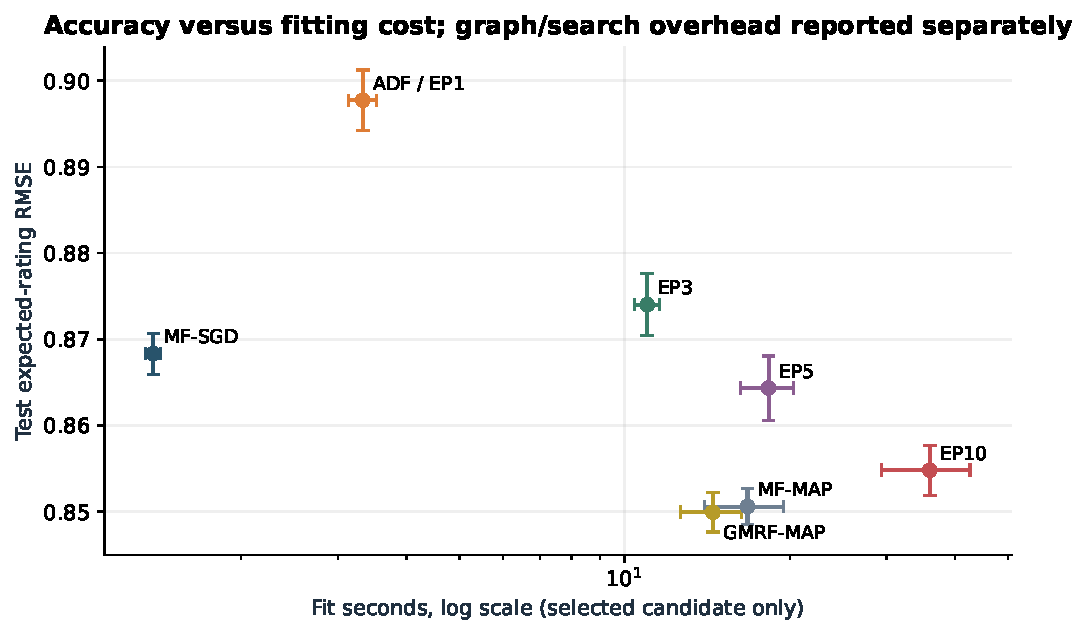
\includegraphics[width=.94\linewidth]{../../Results/analysis/plots/cost_tradeoff.pdf}
\caption{Prediction error versus fitting time. Points omit graph building and
search overhead, which are stated explicitly in the text and raw results.}
\end{figure}

\begin{figure}[!htbp]\centering
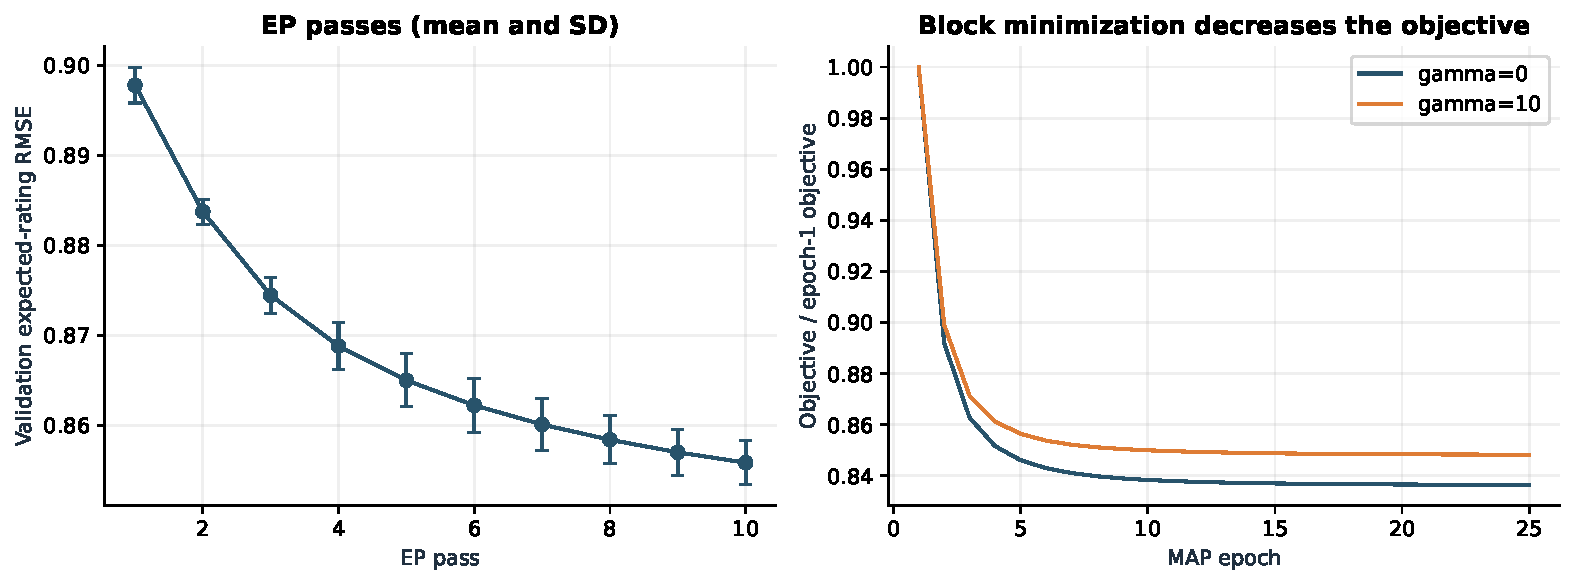
\includegraphics[width=\linewidth]{../../Results/analysis/plots/convergence.pdf}
\caption{Validation error by EP pass and relative MAP objective by epoch.
Lower energy does not guarantee lower held-out error, so validation selects
checkpoints. EP is not claimed to optimize this MAP energy.}
\end{figure}

At EP pass 10, mean RMS parameter change remains 0.01564, despite no skipped
updates in the main EP traces. The local cap is reached by an average of 8.8
updates out of 800,167 at that pass. Stable local calculations therefore do not
establish that the outer posterior approximation has converged.

A separate 12-variable Gaussian Markov diagnostic compares a dense exact
Gaussian solve, Gauss--Seidel MAP iterations and Gibbs sampling. The diagnostic uses a 12-node chain with an extra edge of weight 0.5 between
zero-based nodes 2 and 8, $J=0.8I+2L+\operatorname{diag}(d)$ with $d$
evenly spaced from 0.2 to 1.5, and $h_i=\sin(i+0.4)$.
For $p(q)\propto\exp(-q^TJq/2+h^Tq)$, the known
posterior has mean $J^{-1}h$ and covariance $J^{-1}$. Gauss--Seidel approaches the
exact mean; Gibbs estimates both means and variances with Monte Carlo error.
Increasing sample budget reduces error on average but not necessarily for
every seed. These are additional inference approaches on a tractable
diagnostic, \textbf{not full MovieLens recommender scores}.

\begin{table}[!htbp]\centering\small
\begin{tabular}{@{}lrrrr@{}}\toprule
Method & Budget & Mean RMSE & Variance RMSE & Time (ms)\\\midrule
ExactGaussian & 1 & 0 & 0 & 1.258\\
GaussSeidelMAP & 1 & 0.138 & -- & 0.018\\
GaussSeidelMAP & 5 & 0.00251 & -- & 0.007\\
GaussSeidelMAP & 20 & 4.46e-08 & -- & 0.014\\
GaussSeidelMAP & 100 & 2.17e-17 & -- & 0.066\\
Gibbs & 1000 & 0.0185 & 0.0134 & 2.652\\
Gibbs & 5000 & 0.0111 & 0.00689 & 8.790\\
Gibbs & 20000 & 0.00383 & 0.00333 & 36.379\\
\bottomrule\end{tabular}

\caption{Small Gaussian diagnostic. Gibbs values average five chains/seeds;
1,000 burn-in sweeps are excluded from the sample count but included in time.
MAP has no variance estimate, hence ``--''. Exact/iterative timings are single
small-system measurements. Full variation is in the CSV.}
\end{table}

The original bilinear ordinal quadrature diagnostic is also rerun. It exposes
the same variance/covariance limitations of the factorized approximation;
success on the Gaussian diagnostic does not make bilinear ordinal EP exact.
For a dense $n$-variable Gaussian model, direct solution costs $O(n^3)$,
while a dense iterative or Gibbs sweep costs $O(n^2)$; sparse neighbours
can reduce sweep work. Those guarantees do not turn the full bilinear ordinal
posterior into a Gaussian linear system.
